\begin{frame}{What is an antibody ?}
    \begin{figure}
        \centering
        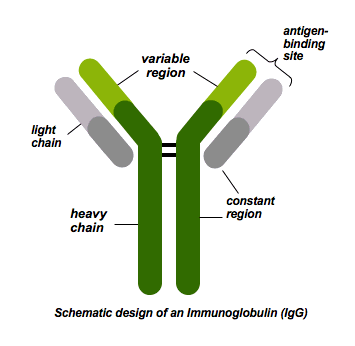
\includegraphics[width=0.5\textwidth]{../Images/schematics_antibody.png}
        \caption{Schematics of an antibody}
        \label{fig:schematics_antibody}
    \end{figure}
\end{frame}

\begin{frame}{What is an antibody ?}


    \begin{figure}
        \centering
        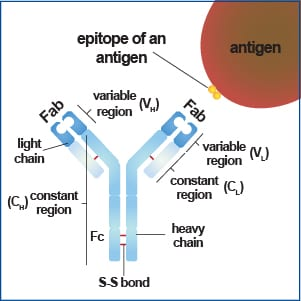
\includegraphics[width=0.5\textwidth]{../Images/antibody_on_antigen.jpg}
        \caption{An antibody binding on an antigen}
        \label{fig:antibody_on_antigen}
    \end{figure}
\end{frame}


\begin{frame}{What is an antibody ?}

    

    \begin{block}{High-specificity binding}
        
        The tip is highly variable to recognize a wide range of antigens
    \end{block}

    \begin{block}{Different types of antibodies}
        \begin{itemize}
        \item The trunk of the antibody is relatively constant 
        \item The small variability creates different antibodies class :\\
        \item[] IgA, IgD, IgE, IgG, or IgM.
        \end{itemize}

    \end{block}
    
\end{frame}